%%%%%%%%%%%%%%%%%%%%%%%%%%%%%%%%%%%%%%%%%%%%%%%%%%%%%%%%%%%%%%%%%%%%%%%%%%%%%%%
% DCC 2027 manuscript rewritten from audited existing experiments, 2026-09-16.
%%%%%%%%%%%%%%%%%%%%%%%%%%%%%%%%%%%%%%%%%%%%%%%%%%%%%%%%%%%%%%%%%%%%%%%%%%%%%%%
\documentclass[smallabstract,smallcaptions]{dccpaper}
\usepackage{amsmath,amssymb,booktabs,graphicx,multirow,url,IEEEtrantools}
\usepackage[hidelinks]{hyperref}
\hypersetup{pdftitle={Rank Before You Merge: Native-Unit Selection for Visual Token Compression},pdfauthor={Zhengxing Yan, Hao Sun, Chen Guo, Jianpeng Hu}}
\begin{document}
\bstctlcite{dccBSTcontrol}
\title{\large\textbf{Rank Before You Merge: Native-Unit Selection\\
for Visual Token Compression}}
\author{\shortstack{
Zhengxing Yan$^{1}$, Hao Sun$^{2}$, Chen Guo$^{3}$, and Jianpeng Hu$^{1,*}$\\[0.4em]
{\small $^{1}$Shanghai University of Engineering Science}\\
{\small $^{2}$Nanjing University of Science and Technology}\\
{\small $^{3}$East China Normal University}\\[0.2em]
{\small \texttt{super\_fw@163.com}; \texttt{sh1076849939@163.com}}\\
{\small \texttt{guochenjkhjk@qq.com}; \texttt{mr@sues.edu.cn}}\\
{\small $^{*}$Corresponding author}}}
\maketitle
\thispagestyle{empty}

\begin{abstract}
Visual token compression depends on both the retained budget and the representation used to select it. We study this dependence in vision-language models with native spatial mergers. Rank-Before-Merge (RBM) scores complete native units using pre-merger feature norms and keeps their identities aligned with the model's visual streams, without training or changing merger weights. At 25\% retention, RBM exceeds post-merger norm selection on all nine text-dense model--benchmark pairs across Qwen3-VL, Qwen2.5-VL, and InternVL3. These operational comparisons include model-specific feature taps and allocation rules. To reduce the feature-depth confound, a separate full-split Qwen3-VL final-input control scores the main merger's own input: it improves TextVQA by 27.68 percentage points, DocVQA by 4.59 points, and OCRBench by 235/1000, but reduces GQA by 5.64 points. The post score still aggregates main and auxiliary outputs, so this control is not a pure intervention on merger order. Rank disagreement and edge-energy associations characterize the selected evidence; a ranking-swap check verifies path equivalence for a fixed kept set. Comparisons with FastV show complementary task preferences rather than uniform superiority. Code: \href{https://github.com/Code-Yan-ZX/qrbm-vlm}{github.com/Code-Yan-ZX/qrbm-vlm}.
\end{abstract}

\Section{Introduction}
High-resolution images produce long visual sequences in modern vision-language models (VLMs). A common architectural response is a native spatial merger: neighboring patch features are converted into fewer language-model inputs. Additional compression must then decide which of these spatial units deserve a smaller token budget. This decision depends on the scoring representation. A large norm before a learned projection need not remain large afterward, and a downstream selector cannot recover evidence from a unit it discards.

We investigate this choice using a deliberately simple, query-blind norm score. Rank-Before-Merge (RBM) selects complete native units from pre-merger features while retaining native merger weights and downstream interface dimensions. It requires neither training nor a second learned compression module. Its purpose is to expose a useful selection signal while respecting the model's existing spatial topology.

Two questions must be separated. First, does an operational RBM implementation preserve accuracy at the same final token budget as post-merger norm selection? Second, does a later pre-merger tap retain the same direction of effect after removing the early-feature advantage? Our three-model comparison addresses the first question. A separate Qwen3-VL experiment scores the main merger's final-block input while holding sample identities and token counts fixed. It reduces, but does not eliminate, implementation differences because the post score concatenates main and auxiliary-stream outputs. This distinction matters because operational Qwen3-VL RBM scores an earlier tap and prunes multiple visual streams.

\begin{figure}[t]
\centering
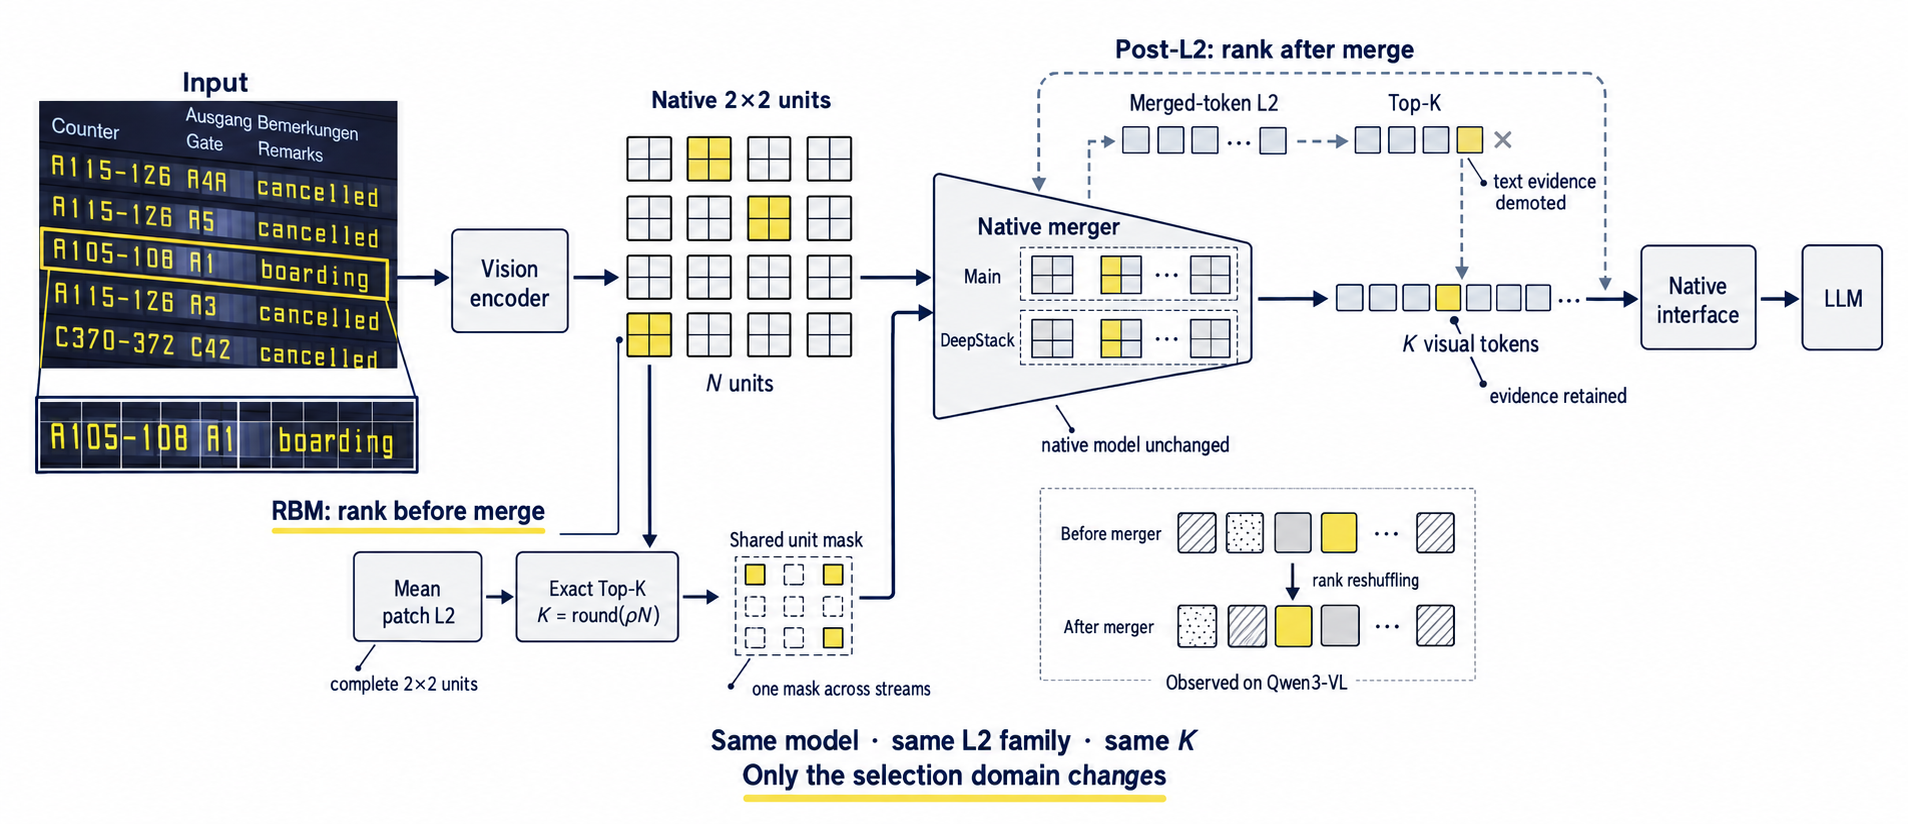
\includegraphics[width=\textwidth]{figs/fig1_user_20260915_v2.png}
\caption{\label{fig:overview}Native-unit selection schematic. Selected identities stay aligned with the surviving visual streams and interface. The illustrated pre-merger location is conceptual: operational Qwen3-VL RBM scores the layer-8 deepstack input, whereas the final-input control scores the main merger's final-block input. The diagram's $\rho$ denotes retention, written $\kappa$ in the text.}
\end{figure}

At 25\% retention, operational RBM improves all nine text-dense comparisons against Post-L2 across three model families. The final-input control also favors its pre-merger score on TextVQA, DocVQA, and OCRBench, but the DocVQA gain is substantially smaller. GQA reverses the direction. Thus neither an architecture-independent preference for earlier features nor a universal advantage over stronger selectors follows from the results.

Our contributions are a native-unit compression rule compatible with deployed merger interfaces; a full-split evaluation separating operational performance from a stricter final-input control; and diagnostics and attention-based comparisons that identify the scope of the observed advantage. We interpret visual-token retention as a task compression budget, without equating it to a bit rate or to total inference cost.

\Section{Related Work}
Visual-token reduction can operate inside the language model through attention or progressive pruning~\cite{chen2024fastv,xing2024pyramiddrop,zhang2024fastervlm,zhang2024sparsevlm}, or at the encoder output through [CLS] attention, graph propagation, fitted predictors, and multiple cues~\cite{wang2024vtccls,shang2024prumerge,ye2024fitprune,jiang2025gprune,luan2025adaptprune}. Unified systems combine saliency with diversity or text guidance~\cite{yu2026visiontrim,baek2026agilepruner,fang2026prunesid}. Their signals and pruning stages differ from RBM's image-only norm score, and equal final token count need not imply equal computation.

Merging changes the representation rather than only deleting tokens. ToMe, VisionZip, and AdaptMerge use matching, dominant-token preservation, and language guidance~\cite{bolya2023tome,yang2024visionzip,islam2025adaptmerge}; TokenPacker learns a compact projector, while GlimpsePrune, VScan, and AnchorPrune adapt reduction to inputs or model families~\cite{li2024tokenpacker,zeng2025glimpseprune,zhang2025vscan,oh2026anchorprune}. These methods motivate treating the selector's input representation as part of the compression rule.

Recent selectors move reduction earlier or vary it across tokens and layers~\cite{gao2026quietprune,wang2026pixelprune,li2026transprune,chen2026v2drop,sun2026hiloprune}; optimize coverage, reconstruction, or sensitivity~\cite{ma2026apet,xu2026score,du2026coin,kim2026zooprune,lee2026spare}; and model semantics, information flow, or head importance~\cite{wang2026metacompress,song2026evocomp,sun2026ifprune,zhu2026hawk}. Layerwise, object-centric, local/global, and hybrid designs preserve evidence in other ways~\cite{wang2026informationhorizon,chen2026alvts,li2026crisp,lei2026core,li2026aot,zhang2026hybrid}. Document pruning and provenance audits expose OCR-specific failures~\cite{choi2026docprune,liu2026provenance}, while LMMs-Eval and EffiVLM-Bench support broader evaluation~\cite{zhang2024lmmseval,wang2025effivlmbench}.

We focus on architectures with native spatial compression: Qwen2.5-VL, Qwen3-VL, and InternVL3~\cite{bai2025qwen25vl,bai2025qwen3vl,zhu2025internvl3}. RBM retains their learned native operators and selects complete input units. Post-L2 is a diagnostic baseline from the same feature-magnitude family; FastV supplies a stronger attention-based comparison. The resulting evidence concerns these implementations and workloads, rather than a claim that downstream selectors generally assume rank preservation or that RBM ranks the full design space above.

\Section{Native-Unit Compression}
\SubSection{Selection representation and token budget}
Let an image contain $N$ native spatial units, each grouping four patch vectors. At retention $\kappa$, retain
\begin{equation}
k=\max\{1,\operatorname{round}(\kappa N)\}.
\end{equation}
For features $h^{(t)}_{u,j}$ at tap $t$, RBM uses
\begin{equation}
a_u^{(t)}=\frac{1}{4}\sum_{j=1}^{4}\|h^{(t)}_{u,j}\|_2,
\qquad K_{\mathrm{RBM}}=\operatorname{TopK}_k\{a_u^{(t)}\}.
\label{eq:pre}
\end{equation}
Post-L2 instead scores a returned visual vector $z_u$:
\begin{equation}
b_u=\|z_u\|_2,\qquad
K_{\mathrm{post}}=\operatorname{TopK}_k\{b_u\}.
\label{eq:post}
\end{equation}
Both rules use magnitude, but they evaluate different representations; they are not identical scoring functions applied to identical vectors. In Qwen3-VL, $z_u$ concatenates the main and three deepstack outputs, whereas the other tested paths use their model-specific post-projector vectors.

In the idealized single-stream case with $h^{(t)}$ at the merger input, $z_u=M(h^{(t)}_{u,1:4})$. For a per-unit merger and a fixed kept set, selection can be performed before or after $M$ without changing the retained outputs. In contrast, the ranking decisions coincide only when their top-$k$ sets agree. A strictly increasing map $b_u=g(a_u)$ is sufficient for agreement at all budgets, but is not a property we assume of learned mergers. We quantify set agreement with Jaccard overlap, $|K_{\mathrm{pre}}\cap K_{\mathrm{post}}|/|K_{\mathrm{pre}}\cup K_{\mathrm{post}}|$. Low overlap alone predicts neither which set is more useful nor the size of an accuracy difference. Qwen3-VL's concatenated post vector departs from this single-stream idealization, so its final-input experiment is a stricter control rather than exact causal isolation.

\SubSection{Model-specific implementation}
RBM retains complete units and keeps selected features aligned with the positions and auxiliary streams expected by each adapter. Model weights, merger weights, interface dimensions, and decoding are unchanged. The implementations follow their backend's compressed-position convention; this does not imply that every backend gathers the selected units' original spatial coordinates. L2 scoring costs $O(Nd)$ for feature dimension $d$; top-$k$ can be implemented in $O(N\log k)$ with a heap. The method adds no learned parameters or language-model attention pass.

For Qwen3-VL, operational RBM scores the first deepstack input at ViT layer~8 and applies one kept set to the main and three deepstack mergers. Post-L2 scores the concatenated returned vector. Consequently, their operational comparison changes feature depth, score aggregation, and where auxiliary streams are pruned. Qwen2.5-VL scores the main merger input, but its available pre path keeps units in window order while the post path follows the native output restoration. InternVL3 scores the concatenated four-patch vector after parameter-free pixel shuffle and before its learned projector; RBM allocates a quota per tile, whereas Post-L2 pools each image's tiles before top-$k$. These results are therefore operational accuracy comparisons, not isolated cross-model merger effects.

The separate Qwen3-VL \emph{Pre-final} control scores final ViT-block features at the main merger input. Pre-final and Post-L2 both execute the deepstack mergers in full and select corresponding rows afterward. Their configuration, sample identities, and per-image token counts match. This removes the early-tap difference, but the pre score still uses four input patch norms while Post-L2 uses a concatenated main-plus-deepstack vector. We therefore call it a final-input control, not a pure stage intervention. It is also not an efficiency measurement of physically skipping merger work, and RBM--Pre-final differences are not pure feature-depth effects.

\Section{Evaluation Protocol}
We evaluate Qwen3-VL-8B, Qwen2.5-VL-7B, and InternVL3-8B with bf16 weights and greedy decoding. The main matrix and final-input control use vLLM 0.19 V1~\cite{kwon2023vllm}. FastV and the hybrid probe use HuggingFace eager attention. We compare methods within each backend; small checks matching native outputs on 8/8 examples and HF/vLLM outputs on 16/16 examples do not establish full-split backend equivalence.

The full evaluation sets contain 5,000 TextVQA examples, 5,349 DocVQA examples, 1,000 OCRBench examples, and 12,578 GQA examples. Metrics are VQA accuracy, ANLS, OCRBench score out of 1,000, and normalized exact match, respectively~\cite{singh2019textvqa,mathew2021docvqa,liu2024ocrbench,hudson2019gqa}. Scoring follows the corresponding lmms-eval rules~\cite{zhang2024lmmseval}. The three former benchmarks are designated text-dense; GQA provides an object-centered question-answering contrast.

All reported compression comparisons retain 25\% of native units and match per-image final visual-token counts within each experiment. Qwen3-VL final-input runs use native image resolution, at most 32 generated tokens, and eager vLLM execution. TextVQA, OCRBench, and GQA use a maximum sequence length of 8,192 and up to eight concurrent sequences; DocVQA uses 32,768 and up to four. Both control arms complete every evaluation sample. The reused uncompressed Qwen3-VL anchors score two TextVQA and 18 OCRBench context overruns as zero. Qwen2.5-VL's operational OCRBench pair uses a shared four-million-pixel cap. InternVL3 DocVQA also uses a four-million-pixel cap. Absolute scores across model families are therefore not controlled model rankings.

For the final-input control, 95\% confidence intervals use 20,000 paired-bootstrap resamples of per-example official scores. We report these intervals separately from the exploratory hybrid probe, for which we make no significance claim. Full-split scores, fixed-size probes, and skipped-example handling are distinguished below.

\Section{Results}
\SubSection{Operational accuracy across model families}
Table~\ref{tab:main} compares the deployed RBM design with Post-L2. RBM improves all nine text-dense model--benchmark pairs: 11.0--38.4 percentage points on TextVQA and DocVQA, and 298--432 points on OCRBench. It nevertheless remains lossy relative to the uncompressed models. For example, Qwen3-VL DocVQA falls from .956 to .481, despite its advantage over Post-L2. A favorable relative comparison is not equivalent to preserving the original model's accuracy.

\begin{table}[t]
\centering
\caption{\label{tab:main}Full-split operational results at 25\% retention. None is uncompressed. Qwen3-VL RBM uses the early tap; this table does not isolate scoring stage. Deltas use unrounded scores and are percentage points except for OCRBench (/1000).}
\small
\setlength{\tabcolsep}{4pt}
\begin{tabular}{llrrrr}
\toprule
Model & Benchmark & None & RBM & Post-L2 & $\Delta$\\
\midrule
\multirow{4}{*}{Qwen3-VL}
& TextVQA & .844 & .605 & .222 & +38.4\\
& DocVQA & .956 & .481 & .238 & +24.3\\
& OCRBench & 760 & 547 & 184 & +363\\
& GQA & .616 & .449 & .477 & $-2.8$\\
\midrule
\multirow{4}{*}{Qwen2.5-VL}
& TextVQA & .862 & .702 & .442 & +26.1\\
& DocVQA & .949 & .636 & .526 & +11.0\\
& OCRBench & 817 & 480 & 182 & +298\\
& GQA & .604 & .559 & .585 & $-2.6$\\
\midrule
\multirow{4}{*}{InternVL3}
& TextVQA & .8338 & .7890 & .4148 & +37.4\\
& DocVQA & .9221 & .7284 & .3820 & +34.6\\
& OCRBench & 852 & 753 & 321 & +432\\
& GQA & .6293 & .5993 & .6031 & $-0.4$\\
\bottomrule
\end{tabular}
\end{table}

GQA favors Post-L2 in all three point estimates. The small InternVL3 difference has an interval crossing zero in the paired analysis. The Qwen results give clearer evidence of a task boundary: pre-merger magnitude is useful for the tested text-dense workloads, but is not a general-purpose saliency criterion.

\SubSection{Final-input control}
Table~\ref{tab:stage} and Fig.~\ref{fig:controls} separate the Qwen3-VL final-input contrast from the operational early-tap design. Pre-final improves TextVQA by 27.68 points and OCRBench by 235/1000. DocVQA improves by 4.59 points, compared with the 24.3-point operational contrast. These are distinct effects; attributing the latter entirely to the main merger boundary would overstate the evidence. Conversely, GQA decreases by 5.64 points in the final-input comparison. The full-split control therefore shows that a later pre-merger representation retains a workload-dependent effect, while its residual score-aggregation difference limits a merger-only attribution.

\begin{table}[t]
\centering
\caption{\label{tab:stage}Qwen3-VL final-input control, complete full splits. Pre-final scores four input patches; Post-L2 scores the concatenated main-plus-deepstack output. Deltas and 95\% paired-bootstrap intervals are percentage points, except OCRBench points.}
\small
\begin{tabular}{lrrr}
\toprule
Benchmark & Pre-final & Post-L2 & $\Delta$ [95\% CI]\\
\midrule
TextVQA & .4985 & .2217 & +27.68 [26.21, 29.19]\\
DocVQA & .2836 & .2377 & +4.59 [3.43, 5.78]\\
OCRBench & 419 & 184 & +235 [199, 271]\\
GQA & .4207 & .4771 & $-5.64$ [$-6.42$, $-4.86$]\\
\bottomrule
\end{tabular}
\end{table}

\begin{figure}[t]
\centering
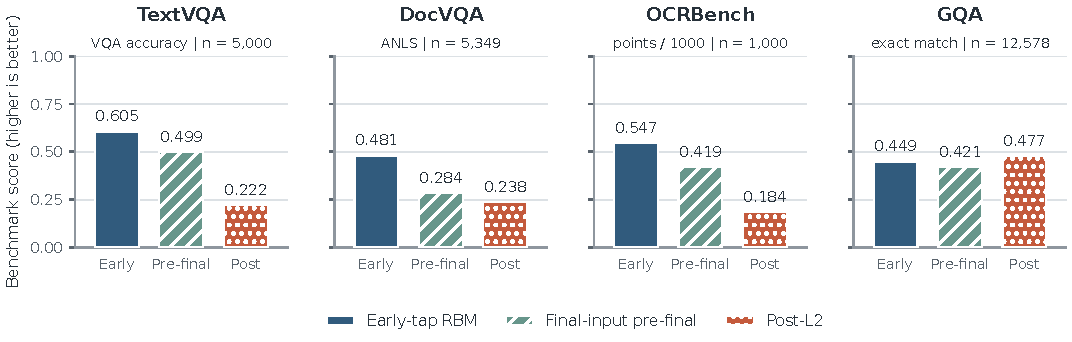
\includegraphics[width=\textwidth]{figs/fig3_fullsplit_controls.pdf}
\caption{\label{fig:controls}Full-split Qwen3-VL accuracy at 25\% retention. Early-tap RBM is the operational design; Pre-final and Post-L2 form the stricter final-input comparison. OCRBench is normalized by 1,000. The RBM--Pre-final difference also includes auxiliary-stream handling and is not a feature-depth-only intervention.}
\end{figure}

\SubSection{Comparison with attention-based selection}
A same-harness full-OCRBench comparison evaluates RBM and FastV-k3 at a shared four-million-pixel cap and a 25\% final budget (Table~\ref{tab:fastv}). Both methods use native positions, greedy decoding, and at most 32 generated tokens. The Qwen3-VL and Qwen2.5-VL runs encounter 79 and 88 common context or memory failures, respectively. These exact shared IDs receive zero in the scores out of 1,000; the completed paired sets contain 921 and 912 examples. RBM leads by 146 and 87 points. These HF scores are a separate experiment and must not be substituted into the vLLM matrix.

\begin{table}[t]
\centering
\caption{\label{tab:fastv}Same-harness HF eager OCRBench comparison, 1,000 attempted examples per model. Common failures are scored zero; both methods retain the same final token count.}
\small
\begin{tabular}{lrrrr}
\toprule
Model & RBM & FastV-k3 & $\Delta$ (/1000) & Completed\\
\midrule
Qwen3-VL & 559 & 413 & +146 & 921\\
Qwen2.5-VL & 382 & 295 & +87 & 912\\
\bottomrule
\end{tabular}
\end{table}

\Section{Diagnostics and Interpretation}
The two operational Qwen3-VL rankings differ substantially. On diagnostic DocVQA, TextVQA, and GQA samples, Spearman correlations are .137, .332, and .360, and top-25\% Jaccard overlaps are .180, .243, and .278. Representation choice therefore changes the selected set, although the different feature depths prevent merger-only attribution.

Rank shifts also associate with local edge energy: post-minus-pre rank correlations with Sobel energy are +.439, +.155, and +.036 in the same task order. On DocVQA, RBM-only versus Post-L2-only units have mean energy .641 versus .124, and 92\% versus 35\% exceed their image's median. Because Sobel energy also responds to borders, texture, and contours, this establishes an edge association rather than text-specific or causal demotion.

A ranking-swap check fixes the post-merger computation but substitutes RBM's kept identities. On the verified Qwen3-VL path, kept-set overlap is 1.000, retained representations are byte-identical, and predictions agree. This verifies path equivalence for a fixed set, not that norm or edge energy identifies causally relevant text. Qwen2.5-VL retains an ordering confound, while InternVL3 provides accuracy-level replication without byte-exact attribution.

\Section{Cost and Limitations}
The retained-unit fraction $k/N$ measures the final visual sequence budget, not an encoded bit rate or total inference cost. FastV processes all candidates through early language-model layers, while RBM does not eliminate vision-transformer work before its scoring tap; Pre-final deliberately executes all merger streams. Resolution, output length, batching, and backend also affect wall-clock performance.

On one A40, a Qwen3-VL TextVQA batch of 200 examples reaches 6.91 requests/s with RBM at 25\% retention, versus 4.11 uncompressed and 6.89 with Post-L2. The vLLM run uses native resolution, at most eight concurrent sequences, greedy decoding capped at 32 tokens, and one untimed warmup; timing excludes engine construction and initial image loading. A separate five-run, one-example proxy averages .23 seconds for RBM and .36 seconds uncompressed. This supports an end-to-end gain for that workload, while the equal RBM/Post-L2 throughput shows no selector-specific speed advantage; the proxy is not a serving-latency distribution.

Our strongest controlled conclusion is the full-split Qwen3-VL final-input comparison, subject to its score-aggregation limitation. The three-model matrix extends the pattern across native merger designs without establishing a universal mechanism. Post-L2 is diagnostic, and FastV shows that RBM is not uniformly strongest. Shared loading failures also limit the HF OCRBench comparison. Broader selectors and direct text-region interventions remain necessary for general competitiveness or semantic claims.

\Section{Conclusion}
Selecting native visual units from pre-merger features is a useful training-free compression design for the tested text-dense workloads. Separating the deployed RBM implementation from a final-input control shows that the useful signal persists at a later pre-merger tap, while score aggregation, feature depth, and stream handling also matter to operational performance. The GQA reversal and FastV comparisons define a clear boundary: selection representation should be evaluated against the intended workload, alongside the token budget and the model's native interface.

\Section{References}
\bibliographystyle{IEEEtran}
\bibliography{references}
\end{document}
